% !TEX root = ../main.tex

\section{Discussion}
Analyzing suggested solutions indicate the following constraints to be satisfied for a sustainable solution:
\begin{enumerate}
	\item Calling \textit{approve} function has to overwrite current allowance with new allowance.
	\item \textit{approve} method does not adjust allowance, it sets new allowance.
	\item Transferring 0 values by \textit{transferFrom} method MUST be treated as normal transfers and fire the \textit{Transfer} event.
	\item Introducing new methods violates ERC20 specifications and it should be avoided for having compatible token with already deployed smart contracts.
	\item Spender will be allowed to withdraw from approver account multiple times, up to the allowed amount.
	\item Transferring initial allowed tokens is considered as legitimate transfer. It could happen right after approval or before changing it.
	\item Race condition MUST not happen in any cases for preventing multiple withdrawal from approver account.\newline
\end{enumerate}
\noindent Comparing suggested solutions shows that they cannot satisfy at least one of the above constraints:
\begin{figure}[h]
	\centering
	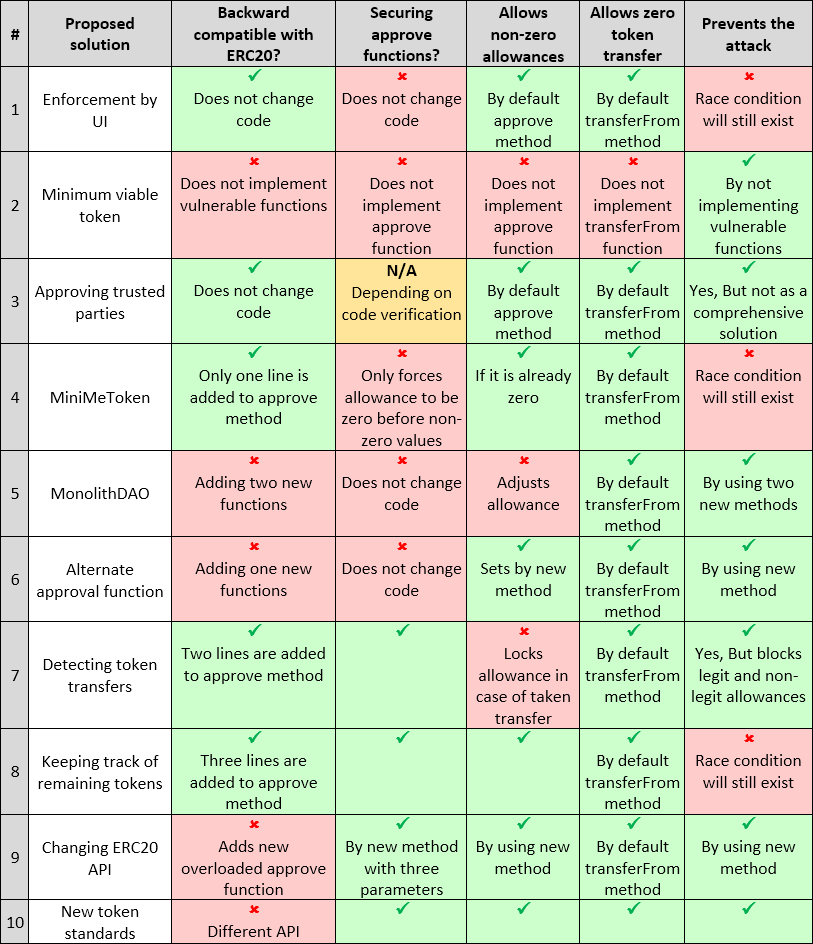
\includegraphics[width=1.0\linewidth]{figures/multiple_withdrawal_27.png}
	\caption{Comparing suggested solutions.}
\end{figure}
\noindent As the comparison table shows, a new solution is required to address this security vulnerability while adhering specification of ERC20 standard. The standard advises approvers to change spender allowance from N to 0 and then from 0 to M (instead of changing it directly from N to M). Since there are gaps between transactions, it would be always a possibility of front-running. As discussed in "MiniMeToken soultion", changing allowance to non-zero values after setting to zero, will require tracking of transferred tokens by the spender. If we can not track transferred tokens, we would not be able to identify if any token has been transferred between execution of transactions. Although It would be possible to track transferred token through \textit{Transfer} events (logged by \textit{transferFrom}), it would not be easily trackable in case of transferring to a third-party (Alice -> Bob, Bob -> Carole => Alice -> Carole). The only solution that removes this gap is to use compare and set (CAS) pattern\cite{Ref06}. It is one of the most widely used lock-free synchronization strategy that allows comparing and setting values in an atomic way. It allows to compare values in one transaction and set new values before transferring control.